\chapter{过程管理}\label{chap:process}

开发期分为三个 Sprint。每轮从需求清单确定交付范围，评审时由组员在运行版本中按角色操作。265 次 Git 提交、34 个 Pull Request、飞书文档和 9 次腾讯会议记录保留了需求决议、返工和复测过程。

\section{Scrum 迭代与工程过程}

\subsection{在一次迭代里走完工程活动}

外送和自取的迭代包含沟通、策划、建模、构建和部署。团队先确认顾客需填写的信息与商家的检查项，再估算工时，在 SRS 和状态图中约定流程。页面与服务合入后，用运行版本走查订单。结算规则有分歧时，回到需求和模型核对。图~\ref{fig:proc-workflow} 展示了这些工作在 Scrum 中的顺序。

\begin{figure}[!htbp]
  \centering
  \resizebox{.92\linewidth}{!}{\begin{tikzpicture}[
  x=1pt,y=-1pt,
  stage/.style={draw=#1!70,fill=#1!7,rounded corners=2pt,line width=.48pt,
    minimum height=28pt,minimum width=93pt,inner sep=3pt,align=center,
    font=\fontsize{10bp}{12bp}\selectfont},
  direction/.style={-{Stealth[length=3.6pt,width=3.1pt]},draw=procink,line width=.6pt},
  annotation/.style={font=\fontsize{8.4bp}{10bp}\selectfont,fill=white,inner sep=1.6pt}
]
  \definecolor{procink}{HTML}{394D59}
  \definecolor{procslate}{HTML}{476C82}
  \definecolor{procsage}{HTML}{397A70}
  \definecolor{procsand}{HTML}{957048}
  \node[stage=procslate] (backlog) at (51,16) {\textbf{Product Backlog}\\REQM 需求基线};
  \node[stage=procslate] (plan) at (161,16) {\textbf{Sprint 规划}\\PP 任务估算};
  \node[stage=procslate] (develop) at (271,16) {\textbf{特性分支开发}\\CM / PMC 日同步};
  \node[stage=procsand] (gate) at (381,16) {\textbf{TDD 与 PR 门禁}};
  \node[stage=procsage] (review) at (51,83) {\textbf{Sprint 评审}\\VAL 增量验收};
  \node[stage=procsage] (retro) at (161,83) {\textbf{Sprint 回顾}\\OPF 过程改进};
  \node[stage=procsage] (release) at (271,83) {\textbf{基线交付}\\VER 归档与部署};
  \draw[direction] (backlog.east) -- (plan.west);
  \draw[direction] (plan.east) -- (develop.west);
  \draw[direction] (develop.east) -- (gate.west);
  \draw[direction] (review.east) -- (retro.west);
  \draw[direction] (retro.east) -- (release.west);
  \draw[direction,rounded corners=3pt] (gate.south) -- (381,115)
    -- node[annotation,pos=.48,above]{575 项测试通过} (51,115) -- (review.south);
  \draw[direction,dashed,draw=procsage] (retro.north)
    -- node[annotation,right,text=procsage]{改进项反哺下轮} (plan.south);
\end{tikzpicture}
}
  \caption{CMM3 过程域与 Scrum 敏捷迭代融合工作流图}\label{fig:proc-workflow}
\end{figure}

一次自取验收中，两端分别通过检查后，团队在评审时走完同一笔订单，验证省略收货地址能否提交。在迭代回顾中，组员再追查为什么两端到联调时才统一规则，并把需要提前确认的条件带入下一轮规划。

\subsection{CMM3 过程域在本项目中的实践映射}

项目沿用 CMM 已定义级强调的过程记录，并按迭代需求裁剪。各端用同一份 SRS 核对规则，每轮更新发生变化的任务、接口和测试，方便成员交接。需求管理、项目策划、验证和确认的对应材料见附录表~\ref{tab:cmm3-mapping}。

调整自取规则时，赵紫怡确认收货地址可省略，并核对订单状态说明。前端结算和后端计价按这一约定修改，再复测外送和自取。版本管理、评审与质量检查贯穿迭代。任务单保存变更内容，PR 记录合入情况，测试核对规则是否落实。

\subsection{需求、迭代与代码怎样交接}

赵紫怡担任 Product Owner，确定需求范围和优先级。李承文担任 Scrum Master，组织迭代，协调阻塞事项、风险和合并检查。四位成员共同交付每轮增量，分别在飞书和 GitHub 记录需求进度与代码评审。图~\ref{fig:proc-repo} 为课程提供的 Gitee 基础仓库，图~\ref{fig:proc-feishu} 为小组的飞书共享空间。

\begin{figure}[!htbp]
  \centering
  \begin{minipage}[t]{.485\linewidth}
    \centering\vspace{0pt}
    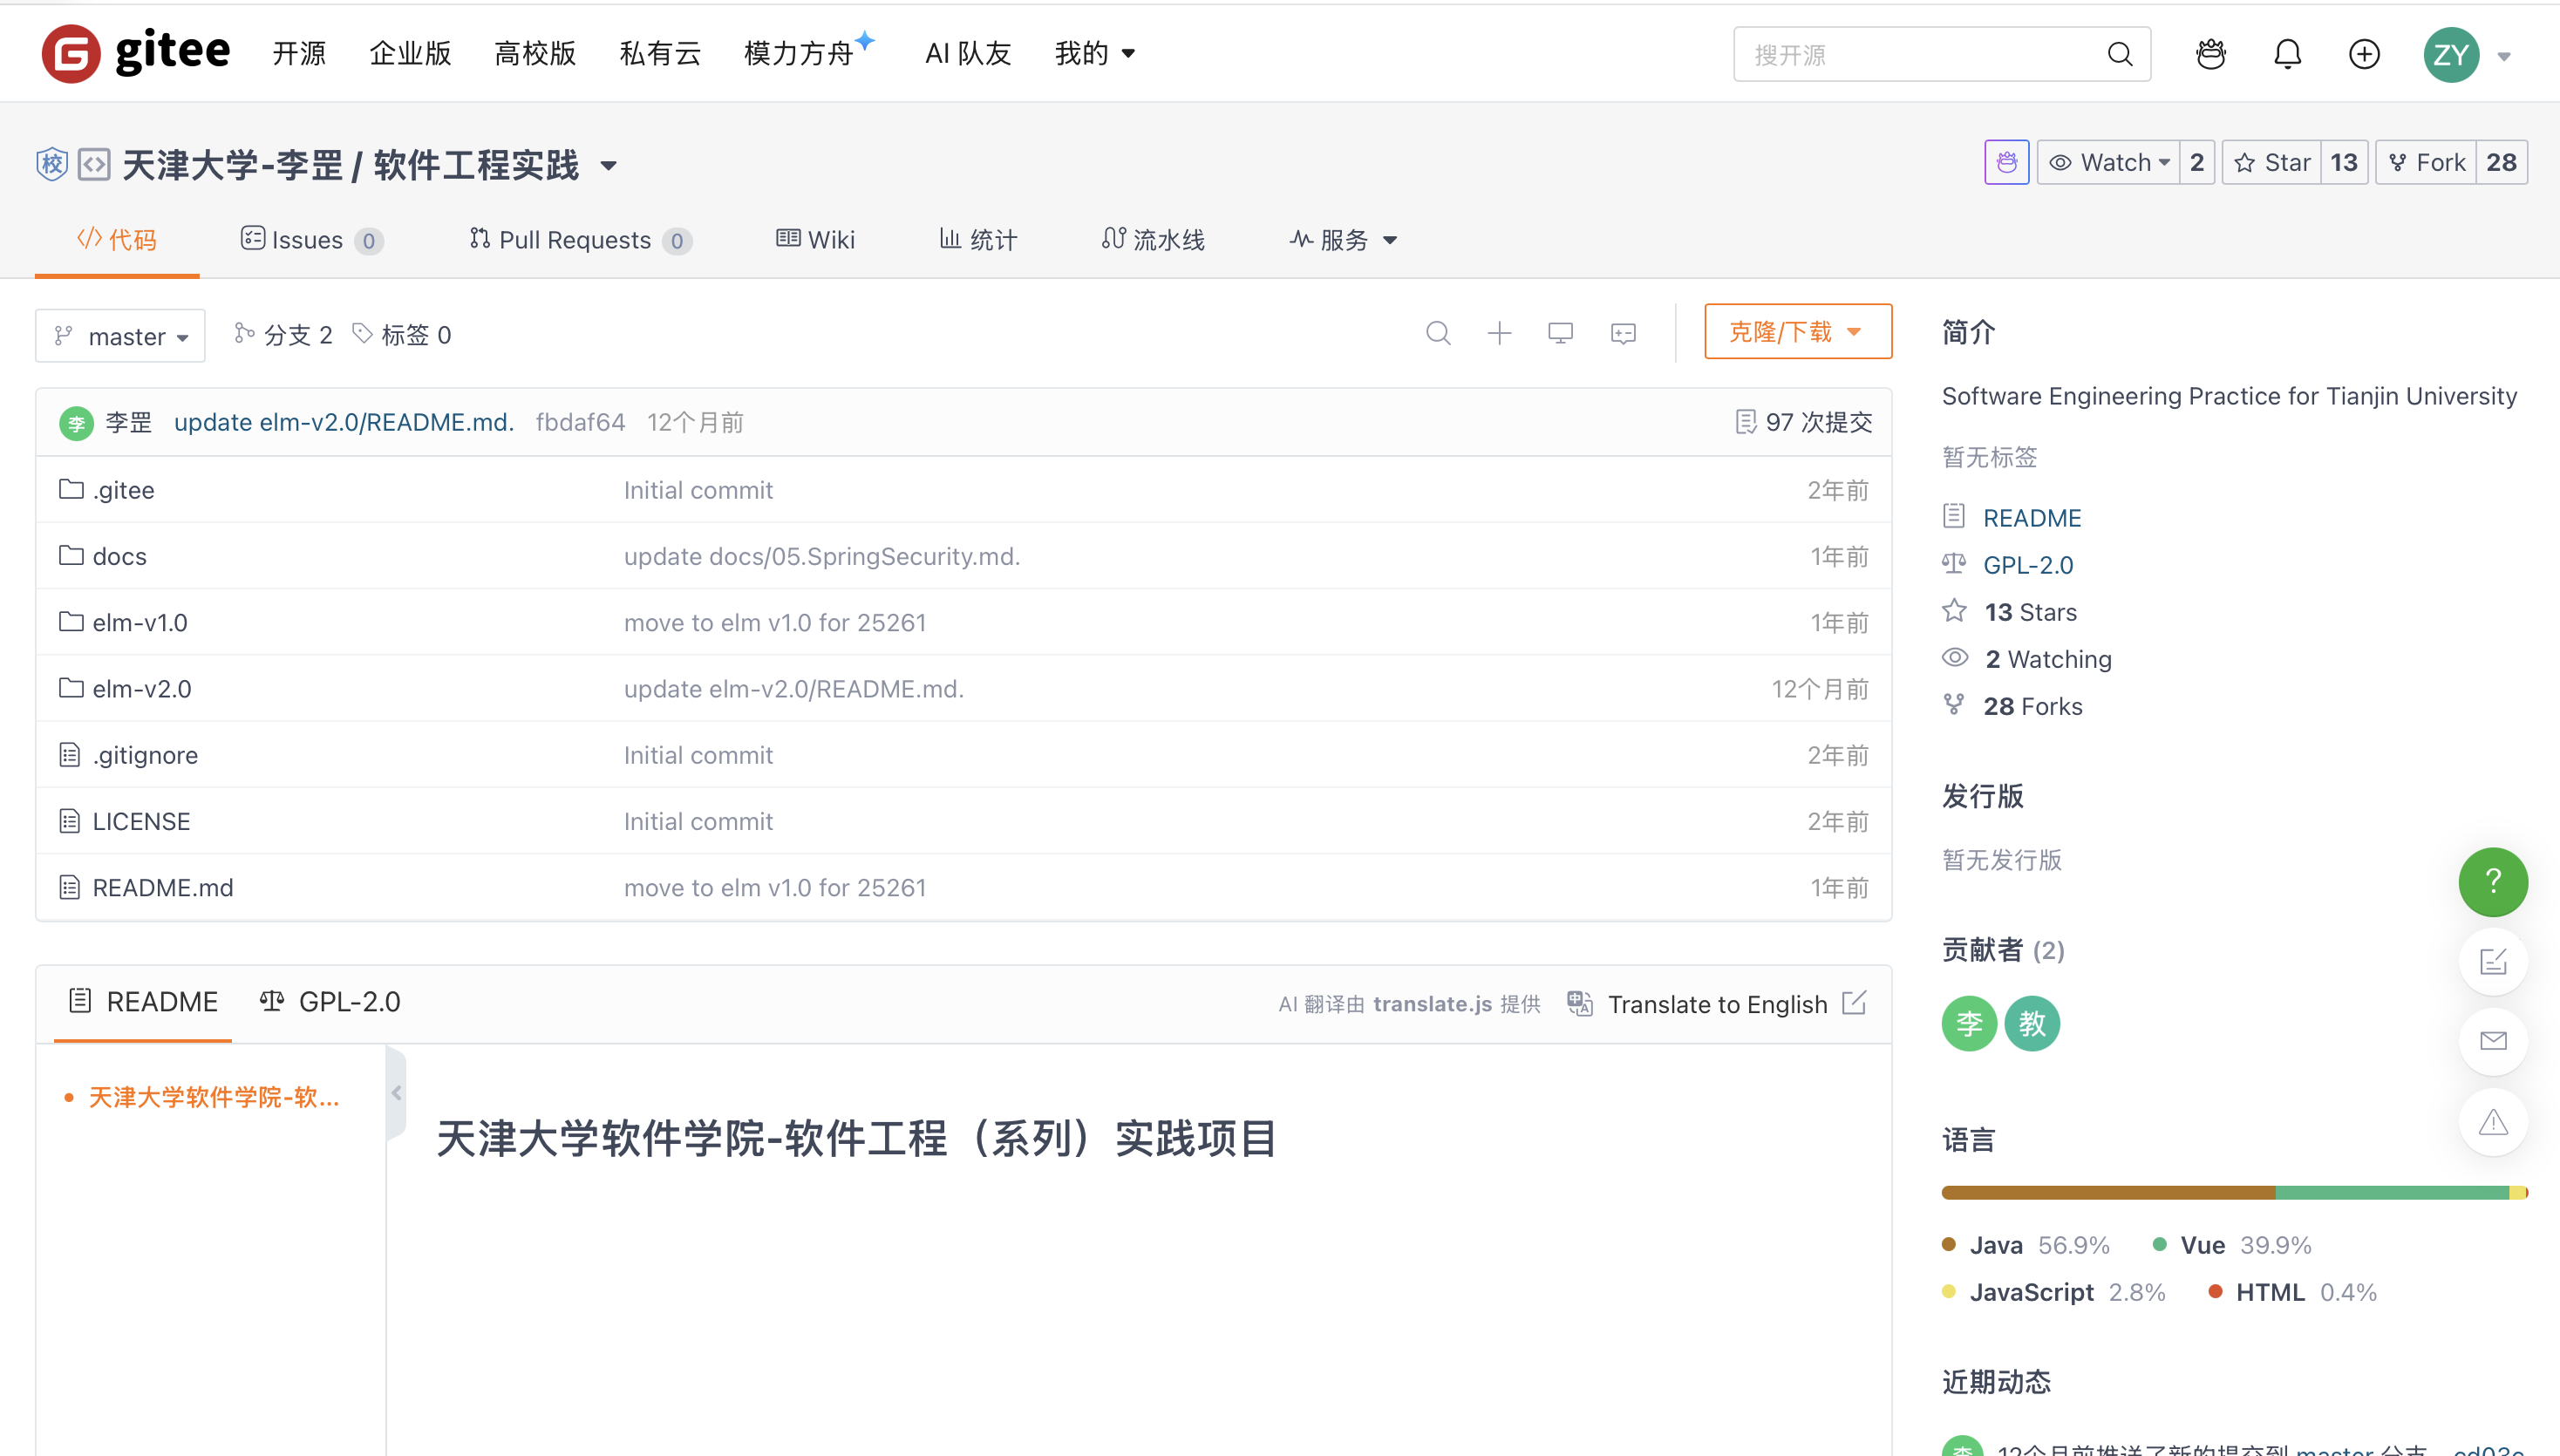
\includegraphics[width=\linewidth,height=.23\textheight,keepaspectratio]{figures/report/process/course-repository.png}
    \captionof{figure}{Gitee 课程仓库分支、目录与提交记录}\label{fig:proc-repo}
  \end{minipage}\hfill
  \begin{minipage}[t]{.485\linewidth}
    \centering\vspace{0pt}
    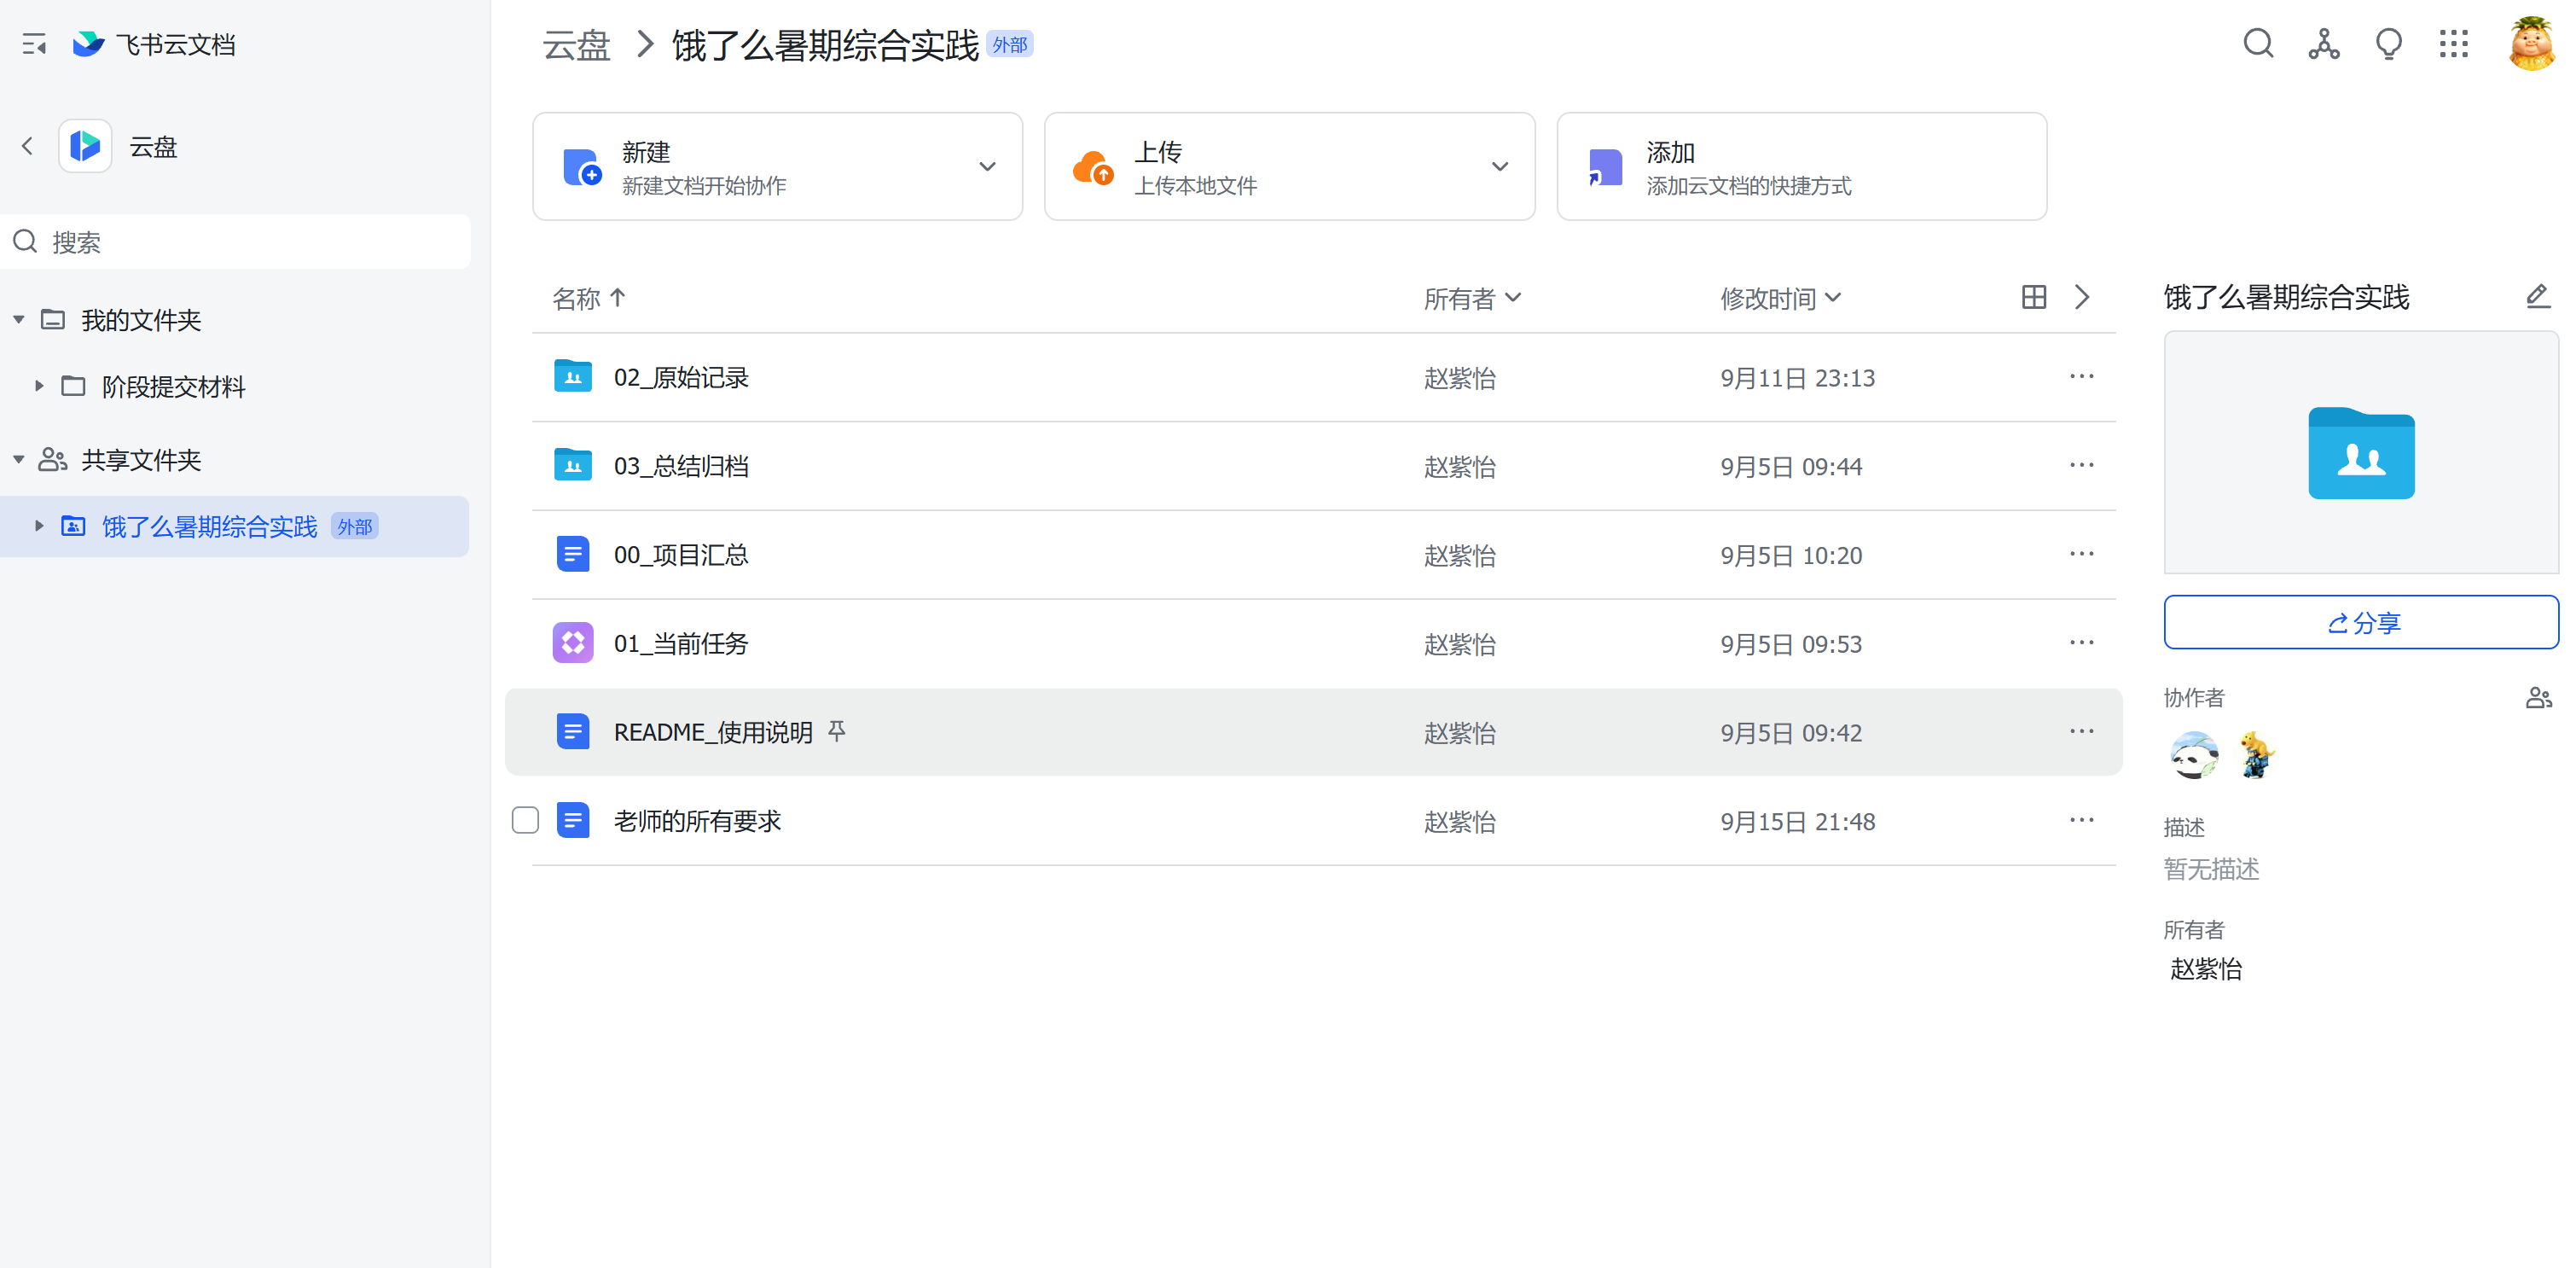
\includegraphics[width=\linewidth,height=.23\textheight,keepaspectratio]{figures/report/process/feishu-workspace.png}
    \captionof{figure}{飞书共享协作空间与任务状态/会议纪要归档视图}\label{fig:proc-feishu}
  \end{minipage}
\end{figure}

\subsection{需求记录与合并检查}

自取规则变更可以从飞书任务追到具体版本。需求单写明负责人和自取结算条件，分支保留计价与页面改动。测试人员分别核对自取与外送，保存下单记录和接口结果，便于追查上次调整的原因。

合并前用 \code{scripts/check-repository.mjs} 检查仓库能否独立检出和部署。检查项包括 README、需求规格、部署说明、相对链接，以及 Compose 引用的挂载文件。部署目标从配置读取，脚本检查个人绝对路径和硬编码部署地址。接口、事务和页面行为由各自的测试覆盖，仓库检查验证交付材料和运行配置能否随项目迁移。

\section{立项组会与阶段会议记录}

\subsection{立项组会快照}

2026 年 9 月 1 日 20:00--21:30，四位成员召开第一次全体会议。李承文主持，赵紫怡在飞书同步记录，范文丽和仲禹潼共同讨论前端页面、角色边界及验收办法。会上确定了项目名称、角色分工、Git 工作流、数据库演进规则和第一轮迭代目标。

\subsection{核心决议}

\begin{reportpoints}
\item 顾客下单和商家履约作为基础，加入骑手配送工作台。地图负责选址与导航，资产模块覆盖模拟钱包、会员、优惠券及积分，多模态 AI 辅助顾客点餐。
\item 后端使用 \code{elm_bk}（Spring Boot 3.4.6、Java 17），前端使用 \code{elmclient}（Vue 3）。成员在特性分支上开发，发起 PR 后由 Scrum Master 复核并合入 \code{main}。
\item 服务端负责核对金额、库存和访问权限。菜品名称和成交单价在下单时写入 \mbox{\code{orderdetailet}}，历史明细读取这份成交记录。
\item 主开发从 9 月 1 日到 9 月 19 日，分为 9 月 1--7 日、8--12 日和 13--19 日三轮。9 月下旬继续整理跨组交叉验收与交付文档。
\end{reportpoints}

\subsection{即时任务分配（RACI 责任矩阵）}

立项时，团队用表~\ref{tab:raci} 明确各项工作的执行（R）、批准（A）、咨询（C）和知会（I）角色。跨成员任务出现分歧时，可按责任矩阵找到确认人。

\begin{table}[H]
  \centering
  \caption{项目核心工程活动 RACI 责任矩阵}\label{tab:raci}
  \reporttablesize
  \begin{tabular}{@{}L{.405\linewidth}C{.135\linewidth}C{.135\linewidth}C{.135\linewidth}C{.135\linewidth}@{}}
\toprule
\textbf{工程活动 / 交付物} & \textbf{范文丽} & \textbf{李承文} & \textbf{赵紫怡} & \textbf{仲禹潼} \\
\midrule
SRS 编写与 UML 建模 & C & C & R/A & C \\
前端四端页面、主题与数据看板 & R/A & C & I & C \\
后端认证、订单、资产与配送接口 & C & R/A & C & I \\
MySQL 表结构与增量迁移设计 & I & C & R/A & I \\
AI 智能点餐与多模态适配 & R & C & R/A & C \\
高德地图选址、距离与导航 & C & C & I & R/A \\
自动化测试、WPS 缺陷台账与\mbox{交叉验收} & C & C & C & R/A \\
Docker 容器编排与 PR 主干合并 & I & R/A & I & C \\
\bottomrule
  \end{tabular}
\end{table}

AI 点餐由赵紫怡和范文丽联调。赵紫怡维护需求和模型接口，范文丽负责输入与展示，李承文核对接口及主干合并，仲禹潼按顾客的操作进行验收。模型不可用时，对照后端返回与页面提示即可定位问题。

菜名快照由赵紫怡确定字段和迁移脚本，李承文核对订单写入和查询，前端与测试再打开历史订单。验收条件是商家改名后，顾客仍能看到成交时的菜名。发现差异时按写入、查询、显示的顺序排查。

\subsection{阶段线上组会纪要汇总}

开发与验收期间，团队通过站会同步当天工作，另在腾讯会议上召开 9 次专题会，确认跨模块问题。会议列表见图~\ref{fig:proc-meetings}，决议和行动记录见附录表~\ref{tab:meeting-log}。

\begin{figure}[H]
  \centering
  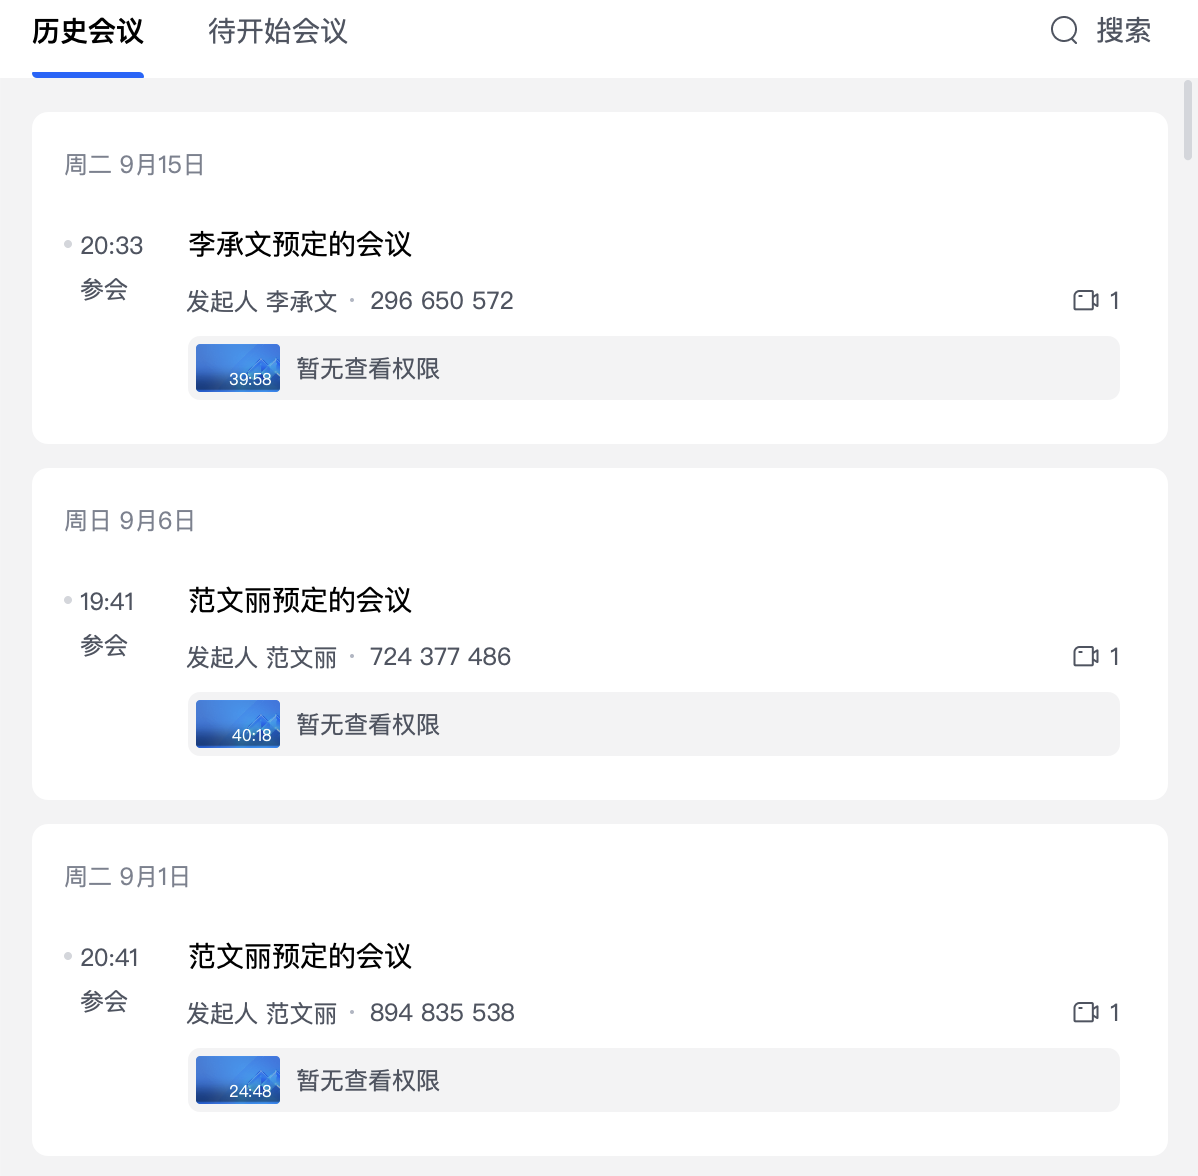
\includegraphics[width=.88\linewidth,height=.50\textheight,keepaspectratio]{figures/report/process/meeting-history.png}
  \caption{团队腾讯会议阶段例会线上历史记录截图}\label{fig:proc-meetings}
\end{figure}

9 月 5 日的接口会统一 JWT 身份、商家和商品字段及订单状态编码。9 月 6 日中期检查处理未登录跳转、字段遗漏和自取规则。第二轮转入多分支合并和公共接口开发。9 月 10 日确定新增接口使用 \code{/api/v1/}，9 月 12 日首次集中联调时，把页面操作、接口响应和后续改动记入同一份 WPS 缺陷台账。9 月 15 日确定封板版本，随后两次会议核对跨组验收发现、演示数据与归档材料。

会后按决议检查合入结果。9 月 10 日确定接口路径后，复查页面实际调用。9 月 15 日封板后，核对 AI 分支、公共外壳及导航修复的合入情况，并复跑 \mbox{原有操作路径}。

\Needspace{.61\textheight}
\section{Sprint 迭代管理}

第一轮交付店铺浏览和下单，第二轮接入商家处理、骑手配送和资产功能，第三轮补充管理端和外部服务。各轮复测已有流程，包括旧订单菜名和页面返回。四类账号的界面见图~\ref{fig:proc-four-roles}，分工和站会记录见附录~\ref{app:process}。

\begin{figure}[H]
  \centering
  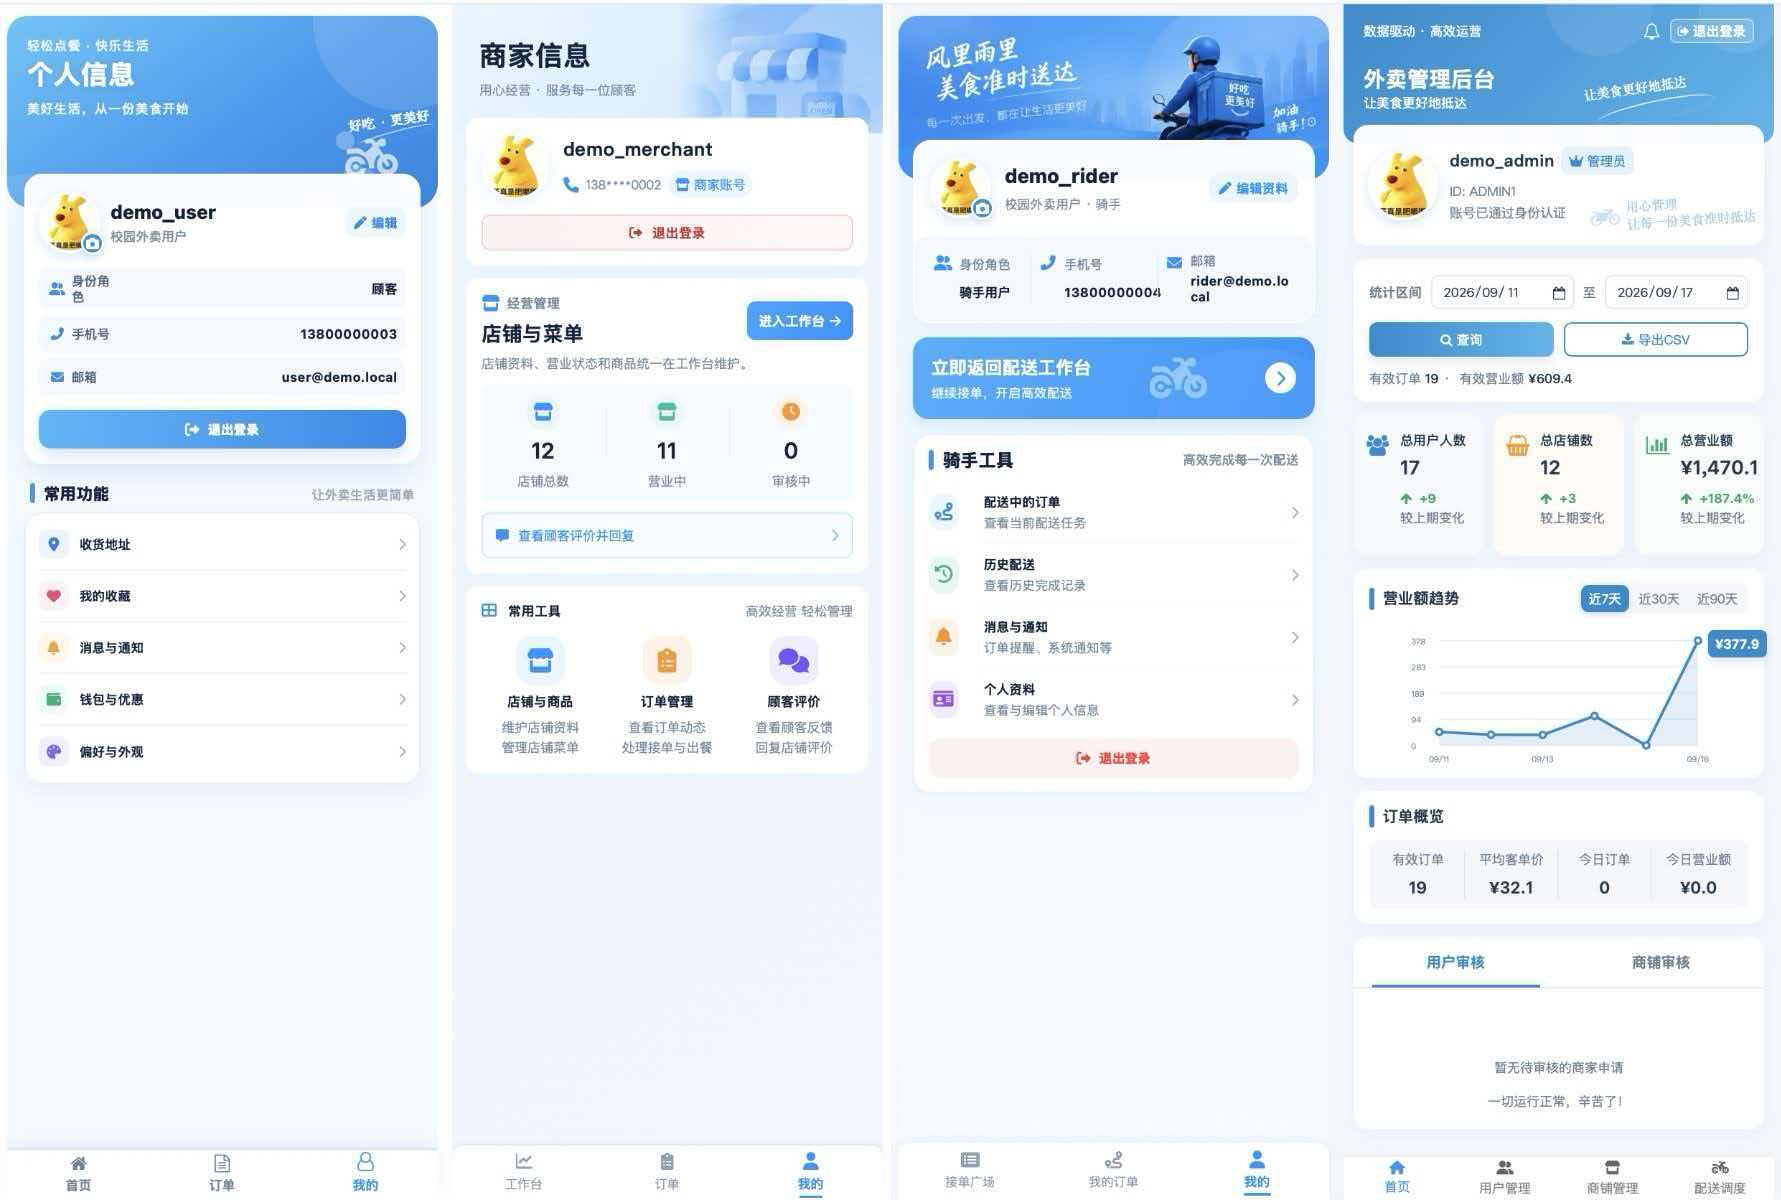
\includegraphics[width=.95\linewidth,height=.46\textheight,keepaspectratio]{figures/report/process/four-roles.jpg}
  \caption{四端核心账号（顾客、商家、骑手、管理员）工作台并行联动效果全景}\label{fig:proc-four-roles}
\end{figure}

顾客从底栏查看订单结果和履约进度。商家在工作台处理本店订单，骑手通过接单广场和配送工作台查看任务，管理员在首页查看平台数据并进入审核与调度。最终联调沿\textbf{同一订单编号}检查四端的操作权限和状态变化，完成履约验收。

\subsection{Sprint 1 需求建模、基础认证与顾客下单核心闭环（9 月 1 日--9 月 7 日）}

\subsubsection{迭代目标与任务拆解}
第一轮计划交付 42 个故事点，投入 80 小时，任务见表~\ref{tab:sprint1-tasks}。团队先确定 SRS 和数据库基线，再实现顾客侧 P0 最小可用版本。首轮评审覆盖游客浏览店铺和菜单，以及登录后的加购、下单、查单和取消。

\subsubsection{每日站会与工作日志（问题与解决过程）}
9 月 3 日和 9 月 7 日是本轮两个集中提交点，分别有 60 次和 35 次提交，主要涉及建模文档和基础认证、编排。附录表~\ref{tab:sprint1-daily} 记录了本轮各日的进展。前半周先把需求写清楚，后半周才有可以连续操作的顾客流程。

团队以 \code{4fcbf00} 初始化课程仓库，并用四端角色组织 SRS 用例。9 月 3 日提交 SRS 初版 \code{6e39d85} 后，大家发现 draw.io 批量导出时有连线错位。统一编号和导出校验后，重新生成了 17 张建模图。接下来清理了构建产物与缓存，统一仓库图片目录，文档可以和代码一道在 PR 中审阅。9 月 6 日的 SRS 2.0 合并保留了已经确认的用例与状态约定，后端骨架和持久化同时继续开发。

首轮联调发现两类交易问题。菜品改名或改价后，历史订单可能读取更新后的商品信息。团队用 \code{003_order_name_snapshot.sql} 补充名称快照，查询改为读取订单明细。回归用例先改商品，再打开原订单，检查成交时的菜名与价格。自取结算起初沿用了外送地址和起送价校验。团队在 \code{OrderPricingService} 中按履约方式计价，前端依据所选方式调整结算项。

9 月 7 日完成认证测试、商铺目录联调和 Docker 基础编排后，评审可以从头操作一次。成员先以游客身份浏览，再登录顾客账号加购，提交订单后检查列表和取消。与规格不一致的步骤会反馈给维护页面、服务或数据库的成员，连同用例编号记录在任务清单。这个顺序也为下一轮商家与骑手接手同一笔订单准备了数据。

首轮按公共目录、登录态、订单提交和回退拆分任务。游客可浏览公共店铺，打开购物车时需要登录。取消订单需校验归属并恢复库存和资产，顾客端按钮随服务端订单状态变化。各项通过后再连续操作一遍，检查登录跳转、页面读写\mbox{和数据状态能否衔接}。

\subsubsection{迭代燃尽图、评审与回顾}
产品负责人和组员共同评审注册、登录、游客浏览、加购、下单与取消，结果见表~\ref{tab:sprint1-review}。快照和自取修复使剩余工时在 9 月 5 日偏离理想线，\mbox{9 月 7 日归零（图~\ref{fig:burndown-s1}）}。

折线在 9 月 4 日至 5 日只下降 3 小时，剩余工作从 45 小时减到 42 小时，是首轮收敛最慢的一段。收尾评审沿顾客流程检查补丁合入后的历史菜名、自取提交和取消时的数据恢复。

\begin{figure}[!htbp]
  \centering
  \resizebox{.86\linewidth}{!}{%
\begin{tikzpicture}[x=1.52cm,y=0.059cm]
    \definecolor{proctrend}{HTML}{25465D}
    \definecolor{procaxes}{HTML}{3F505E}
    \definecolor{procgrid}{HTML}{DFE5E9}
    \foreach \y in {0,20,40,60,80} {
      \draw[procgrid,line width=.4pt] (0,\y) -- (6.72,\y);
      \node[left,font=\scriptsize,text=procaxes] at (0,\y) {\y};
    }
    \draw[procaxes,line width=.52pt] (0,90) -- (0,0) -- (6.72,0);
    \foreach \d/\lbl in {0/9.1,1/9.2,2/9.3,3/9.4,4/9.5,5/9.6,6/9.7} {
      \draw[procaxes,line width=.45pt] (\d,0) -- ++(0,-2.5pt);
      \node[below=3pt,font=\scriptsize,text=procaxes] at (\d,0) {\lbl};
    }
    \node[anchor=south west,inner sep=1pt,font=\scriptsize,text=procaxes] at (0,90) {剩余工时 (h)};
    \node[anchor=north east,inner sep=0pt,font=\scriptsize,text=procaxes] at (6.72,-15pt) {日期 (9月)};

    \draw[procaxes,dash pattern=on 3pt off 2.6pt,line width=.62pt] (0,80) -- (6,0);
    \draw[proctrend,line width=.92pt] plot[mark=*,mark size=1.6pt,mark options={solid,fill=white,line width=.72pt}]
      coordinates { (0,80) (1,70) (2,54) (3,45) (4,42) (5,22) (6,0) };

    \draw[procaxes,dash pattern=on 3pt off 2.6pt,line width=.62pt]
      (4.05,78) -- ++(16pt,0) node[right=3pt,font=\scriptsize,text=procaxes] {理想基准线};
    \draw[proctrend,line width=.92pt] (4.05,69)
      -- ++(16pt,0) node[right=3pt,font=\scriptsize,text=procaxes] {实际剩余工时};
    \draw[proctrend,fill=white,line width=.72pt] (4.235,69) circle[radius=1.6pt];
  \end{tikzpicture}
}
  \caption{Sprint 1 迭代工时燃尽图（9 月 1 日--9 月 7 日，总工时 80 h）}\label{fig:burndown-s1}
\end{figure}

\begin{longtable}{L{.18\linewidth}L{.44\linewidth}L{.29\linewidth}}
\caption{Sprint 1 迭代评审验收与回顾总结表}\label{tab:sprint1-review}\\
\toprule
\textbf{评估维度} & \textbf{核心结论与验收事实} & \textbf{沉淀行动项（Try）} \\
\midrule
增量评审（Review） & \code{US001--US007} 中顾客核心点餐链路全部跑通。完成认证与商品目录 2 轮 TDD 提交。Docker 基础服务可正常启动。 & 在 Sprint 2 全面推行“RED-GREEN-REFACTOR”三步\mbox{提交模式。} \\
过程回顾（Keep/Prob） & 保留飞书任务与 PR 审查节奏。初版接口未对齐自取规则，结算联调中\mbox{补做了调整。} & 新增“业务枚举与状态编码变更必须在组会\mbox{同步后再编码”规范。} \\
\bottomrule
\end{longtable}

\subsection[Sprint 2 商家工作台、骑手配送闭环\texorpdfstring{\protect\newline}{}与资产积分系统（9 月 8 日--9 月 12 日）]{Sprint 2 商家工作台、骑手配送闭环与资产积分系统（9 月 8 日--9 月 12 日）}

\subsubsection{迭代目标与任务拆解}
第二轮计划 40 个故事点、68 小时。商家接单并备餐，骑手领取配送任务，最后由顾客确认收货。沿这条路径，我们把模拟钱包、优惠券、积分、评价和站内通知接进来，也开始整合新的登录页和第一版 AI。任务见表~\ref{tab:sprint2-tasks}。

\subsubsection{每日站会与工作日志（问题与解决过程）}
第二轮验收覆盖整条履约链路。商家接单备餐，骑手在任务池接单，依次到店、取餐、送达，顾客在订单页查看状态。各端分别刷新列表，统一读取服务端的订单和配送任务状态。9 月 8--12 日的联调记录见附录表~\ref{tab:sprint2-daily}。

两位骑手同时抢单时，后到的请求可能覆盖任务归属。\mbox{\code{delivery_task}} 的条件更新要求任务仍待领取且尚未分配骑手。领取成功后递增 \mbox{\code{version}}，只有更新成功的一方取得任务。页面按服务端响应刷新任务池，商家和顾客继续跟踪同一订单。9 月 9 日补测了订单名称快照，商家修改商品资料后可用同一用例复测。

资产与订单联调时发现，重复请求可多次领取新人券。团队在领券操作中加入判重和唯一领取校验。钱包余额、积分和优惠券用于模拟支付，验收时对照顾客结算、资产流水和取消后的恢复结果。业务修复与回归用例一同合入，供下一轮\mbox{整合管理端时复跑}。

登录页视觉和 AI 入口调整都涉及前端的公共区域。范文丽把登录页背景移到独立作用域，并补上视觉回归检查。请求经过登录状态判断后，游客仍可浏览公共页面。9 月 12 日的四端联调发现了返回循环、窄屏溢出等问题。团队在 WPS 台账中记下入口和操作顺序，附上截图，并把跨页面修复列入 Sprint~3。

第二轮验收在多类账号之间切换。商家查看待处理订单，订单达到可配送状态后骑手端才显示任务，顾客随后核对进度。一端刷新延迟也会阻碍下一步操作。联调记录同时写明操作方和期望状态。发现页面与接口响应不同步时，先查订单当前状态，再定位客户端展示或服务端动作。

\subsubsection{迭代燃尽图、评审与回顾}
这一轮计划 68 小时。资产事务和登录页样式重构多花了一些工时，实际曲线略偏离理想线，到第 5 天归零。图~\ref{fig:burndown-s2} 记剩余工时，表~\ref{tab:sprint2-review} 记录评审结果与下一轮改进措施。

9 月 10 日尚余 42 小时，比同一时点的均匀计划多 8 小时。之后两天分别降到 20 小时和零，涵盖了从各端各自开发转向集中联调的阶段。此时的完成条件包括任务成功交接，以及页面状态和资产流水能够相互核对。

\begin{figure}[!htbp]
  \centering
  \resizebox{.86\linewidth}{!}{%
\begin{tikzpicture}[x=2.13cm,y=0.067cm]
    \definecolor{proctrend}{HTML}{287B78}
    \definecolor{procaxes}{HTML}{3F505E}
    \definecolor{procgrid}{HTML}{DFE5E9}
    \foreach \y in {0,20,40,60} {
      \draw[procgrid,line width=.4pt] (0,\y) -- (4.72,\y);
      \node[left,font=\scriptsize,text=procaxes] at (0,\y) {\y};
    }
    \draw[procaxes,line width=.52pt] (0,79) -- (0,0) -- (4.72,0);
    \foreach \d/\lbl in {0/9.8,1/9.9,2/9.10,3/9.11,4/9.12} {
      \draw[procaxes,line width=.45pt] (\d,0) -- ++(0,-2.5pt);
      \node[below=3pt,font=\scriptsize,text=procaxes] at (\d,0) {\lbl};
    }
    \node[anchor=south west,inner sep=1pt,font=\scriptsize,text=procaxes] at (0,79) {剩余工时 (h)};
    \node[anchor=north east,inner sep=0pt,font=\scriptsize,text=procaxes] at (4.72,-15pt) {日期 (9月)};

    \draw[procaxes,dash pattern=on 3pt off 2.6pt,line width=.62pt] (0,68) -- (4,0);
    \draw[proctrend,line width=.92pt] plot[mark=*,mark size=1.6pt,mark options={solid,fill=white,line width=.72pt}]
      coordinates { (0,68) (1,54) (2,42) (3,20) (4,0) };

    \draw[procaxes,dash pattern=on 3pt off 2.6pt,line width=.62pt]
      (2.75,68) -- ++(16pt,0) node[right=3pt,font=\scriptsize,text=procaxes] {理想基准线};
    \draw[proctrend,line width=.92pt] (2.75,59)
      -- ++(16pt,0) node[right=3pt,font=\scriptsize,text=procaxes] {实际剩余工时};
    \draw[proctrend,fill=white,line width=.72pt] (2.882,59) circle[radius=1.6pt];
  \end{tikzpicture}
}
  \caption{Sprint 2 迭代工时燃尽图（9 月 8 日--9 月 12 日，总工时 68 h）}\label{fig:burndown-s2}
\end{figure}

\begin{longtable}{L{.18\linewidth}L{.44\linewidth}L{.29\linewidth}}
\caption{Sprint 2 迭代评审验收与回顾总结表}\label{tab:sprint2-review}\\
\toprule
\textbf{评估维度} & \textbf{核心结论与验收事实} & \textbf{沉淀行动项（Try）} \\
\midrule
增量评审（Review） & \code{US008--US016} 商家接单出餐、骑手抢单送达、钱包积分抵扣与评价回复均已联调成功，WPS 缺陷表正式运转。 & 将集中联调暴露的“返回死循环、窄屏溢出”纳入 Sprint 3 优先修复。 \\
过程回顾（Keep/Prob） & 保留订单名称快照的 TDD 回归。登录等跨分支\mbox{样式合并}暴露了全局 CSS \mbox{覆盖冲突。} & Sprint 3 推行页面级主题变量与\mbox{壳层对齐规范。} \\
\bottomrule
\end{longtable}

\subsection{Sprint 3 平台治理、多模态 AI、地图与回归（9 月 13--19 日）}

\subsubsection{迭代目标与任务拆解}
第三轮分到 36 个故事点，计划投入 82 小时。管理员开始用审核、治理和全局看板，顾客端加入文字问答、菜品推荐、识菜和语音点餐，高德地图负责选址与估算距离。四套主题与页面动效也纳入这一版，最后在同一个版本上做全量回归和跨组验收。任务见表~\ref{tab:sprint3-tasks}。

\subsubsection{每日站会与工作日志（问题与解决过程）}
第三轮并行推进管理端审核、看板、AI 和地图。9 月 14--16 日共有 45 次核心提交，包含第 7 次封板会与第 8 次验收准备会提出的变更。附录表~\ref{tab:sprint3-daily} 按阶段列出\mbox{提交和复测线索}。

9 月 13 日调试外部模型时，网络等待延长了数据库事务。团队将\textbf{外部 HTTP 调用移出事务}，设置总超时，并保留本地帮助与规则筛选。9 月 16 日集成地图选址、GCJ-02 坐标距离估算和骑手导航。地图服务不可用时，地址页显示服务状态并提供文本地址与离线区域选择，顾客可继续下单。

\paragraph{页面返回问题的三步修复}
团队在桌面和 375~px 窄屏走查 AI 页、登录和订单页。从 AI 主页面打开工具页后连退两次，有时会绕回 AI。台账记录入口和操作顺序，回归用例用实际路由复现问题。修复后整理各页返回规则和默认入口，再复跑原用例。三步对应的提交见表~\ref{tab:nav-tdd-process}。

\begin{longtable}{L{.17\linewidth}L{.16\linewidth}L{.58\linewidth}}
\caption{Sprint 3 页面返回问题的 TDD 提交}\label{tab:nav-tdd-process}\\
\toprule
\textbf{阶段} & \textbf{提交} & \textbf{验证重点} \\
\midrule
RED & \code{06780ac} & 先用回归用例复现返回循环，明确连续返回两次\mbox{应回到原页面。} \\
GREEN & \code{12c3d6e} & 调整 AI 工具切换与返回逻辑，使工具页面切换复用历史记录，连续返回能够退出。 \\
REFACTOR & \code{d319c5e} & 整理共用导航规则，继续执行路由回归。 \\
\bottomrule
\end{longtable}

课程源码中，\code{navigation.test.mjs} 读取项目的实际路由配置，再模拟浏览历史与各页面的返回处理。除常见的“首页、AI、推荐、依次返回”外，测试还覆盖直接打开语音或识菜页，以及从带筛选参数的商铺列表进入 AI 后返回。前一种情形需要走应用内默认入口，后一种应保留来源页和查询参数。测试从用户动作出发，改动路由或页面组件时也可以继续执行。

同期修复了连续切页白屏、窄屏表单横向溢出和语音抽屉关闭后音轨未释放的问题。首页与分类卡片按 \code{prefers-reduced-motion} 设置减少动画。9 月 16 日完成地图联调与跨组验收，17--19 日归档 25 张交叉验收截图，并执行前后端全量回归。

第三轮在同一版本上核对新增能力和既有流程。管理端验证入驻审核、账号启停和异常处置，顾客端复查浏览、加购和下单。AI 和地图检查功能入口以及服务不可用时的页面响应。接口和页面冻结后集中处理跨端与导航问题，按封板版本归档回归结果与截图。

\subsubsection{迭代燃尽图、评审与回顾}
9 月 15 日集中合入版本时，团队同时处理导航的 TDD 修复，之后剩余工时逐日减少，见图~\ref{fig:burndown-s3}。表~\ref{tab:sprint3-review} 记录了版本验收结果和团队回顾。

9 月 15 日封板时还剩 48 小时，次日降至 26 小时。最后三天的曲线逐步放缓，对应封板后的验收与收尾。表~\ref{tab:sprint3-review} 也记录了这段时间才集中完成的外部服务降级检查，为下一轮提前安排测试环境留下了依据。

\begin{figure}[H]
  \centering
  \resizebox{.86\linewidth}{!}{%
\begin{tikzpicture}[x=1.52cm,y=0.059cm]
    \definecolor{proctrend}{HTML}{A87435}
    \definecolor{procaxes}{HTML}{3F505E}
    \definecolor{procgrid}{HTML}{DFE5E9}
    \foreach \y in {0,20,40,60,80} {
      \draw[procgrid,line width=.4pt] (0,\y) -- (6.72,\y);
      \node[left,font=\scriptsize,text=procaxes] at (0,\y) {\y};
    }
    \draw[procaxes,line width=.52pt] (0,92) -- (0,0) -- (6.72,0);
    \foreach \d/\lbl in {0/9.13,1/9.14,2/9.15,3/9.16,4/9.17,5/9.18,6/9.19} {
      \draw[procaxes,line width=.45pt] (\d,0) -- ++(0,-2.5pt);
      \node[below=3pt,font=\scriptsize,text=procaxes] at (\d,0) {\lbl};
    }
    \node[anchor=south west,inner sep=1pt,font=\scriptsize,text=procaxes] at (0,92) {剩余工时 (h)};
    \node[anchor=north east,inner sep=0pt,font=\scriptsize,text=procaxes] at (6.72,-15pt) {日期 (9月)};

    \draw[procaxes,dash pattern=on 3pt off 2.6pt,line width=.62pt] (0,82) -- (6,0);
    \draw[proctrend,line width=.92pt] plot[mark=*,mark size=1.6pt,mark options={solid,fill=white,line width=.72pt}]
      coordinates { (0,82) (1,68) (2,48) (3,26) (4,14) (5,6) (6,0) };

    \draw[procaxes,dash pattern=on 3pt off 2.6pt,line width=.62pt]
      (4.05,79) -- ++(16pt,0) node[right=3pt,font=\scriptsize,text=procaxes] {理想基准线};
    \draw[proctrend,line width=.92pt] (4.05,70)
      -- ++(16pt,0) node[right=3pt,font=\scriptsize,text=procaxes] {实际剩余工时};
    \draw[proctrend,fill=white,line width=.72pt] (4.235,70) circle[radius=1.6pt];
  \end{tikzpicture}
}
  \caption{Sprint 3 迭代工时燃尽图（9 月 13 日--9 月 19 日，总工时 82 h）}\label{fig:burndown-s3}
\end{figure}

\begin{longtable}{L{.18\linewidth}L{.44\linewidth}L{.29\linewidth}}
\caption{Sprint 3 迭代评审验收与回顾总结表}\label{tab:sprint3-review}\\
\toprule
\textbf{评估维度} & \textbf{核心结论与验收事实} & \textbf{沉淀行动项（Try）} \\
\midrule
增量评审（Review） & \code{US017--US022} 的管理治理、多模态 AI、高德适配与四端看板完成集成，575 项自动化测试通过。 & 形成可一键启动的 Docker 演示镜像与差异演进清单。 \\
过程回顾（Keep/Prob） & 集成前后继续执行 TDD 与契约测试。未配置外部 API 密钥的界面降级测试\mbox{集中在后期完成。} & 后续外部依赖在设计初期即同步定义“降级提示\mbox{与测试替身”。} \\
\bottomrule
\end{longtable}

\FloatBarrier
\Needspace{6\baselineskip}
\subsection{《软件工程 1》过程审计与规范化收尾（9 月下旬--11 月）}

功能验收后，团队按课程要求复核答辩中提出的问题。9 月 23--27 日整理基础技术文档和跨组测试材料，相关改动见 \code{29a0ad1} 至 \code{6ddb219}。

随后在《软件工程 1》阶段，团队按 \code{6ddb219} 快照复跑 575 项前后端自动化测试，在独立的 MySQL 8.0.46 演示实例上核对四端主界面和 AI、地图的降级状态。验收记录按角色、场景和结果归档，与 WBS、PERT 工时、风险记录及 AI 核查材料一起汇入课程报告。

图~\ref{fig:proc-gh-summary} 和图~\ref{fig:proc-prs} 可以按分支和合入请求查回变更。以 9 月 15 日封板为例，先在 PR 记录里查公共壳层和导航修复涉及的改动，再结合当日的会议纪要与回归检查，判断合入版本是否达到进入验收的条件。

\Needspace{.48\textheight}
\begin{figure}[H]
  \centering
  \begin{minipage}[t]{.485\linewidth}
    \centering\vspace{0pt}
    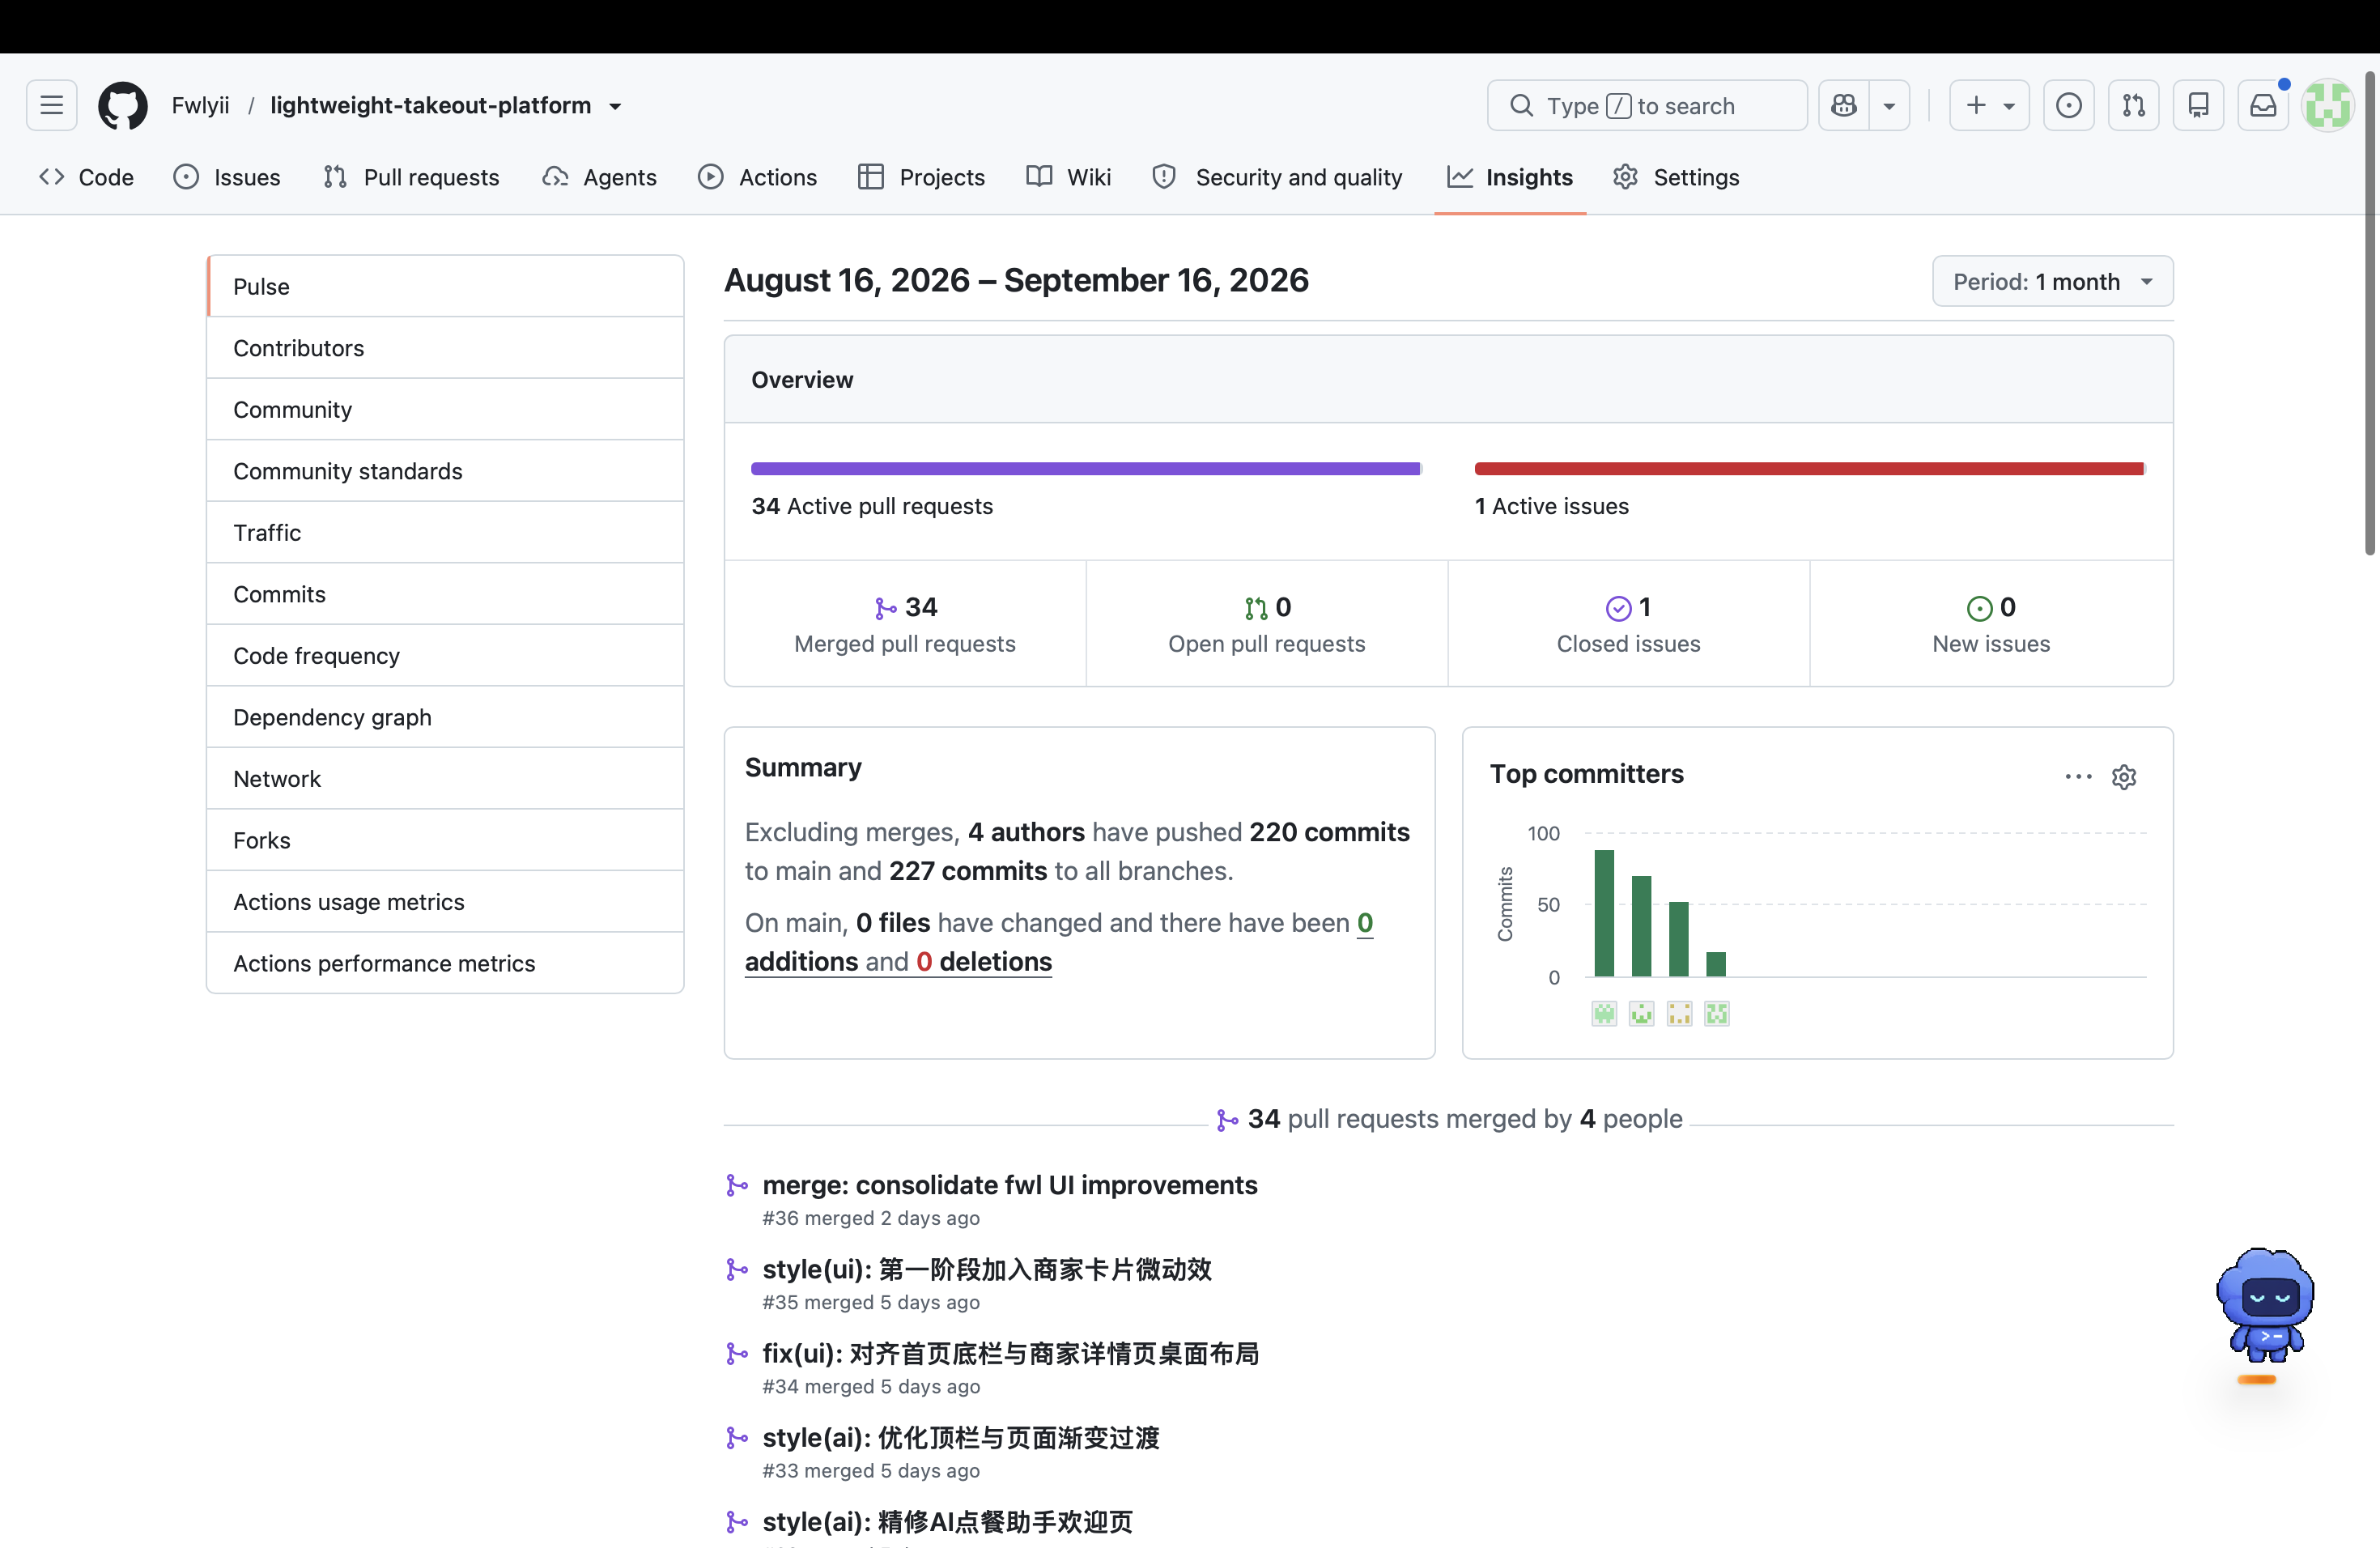
\includegraphics[width=\linewidth,height=.23\textheight,keepaspectratio]{figures/report/process/github-summary.png}
    \captionof{figure}{GitHub 仓库分支合并、提交统计与成员协同全景}\label{fig:proc-gh-summary}
  \end{minipage}\hfill
  \begin{minipage}[t]{.485\linewidth}
    \centering\vspace{0pt}
    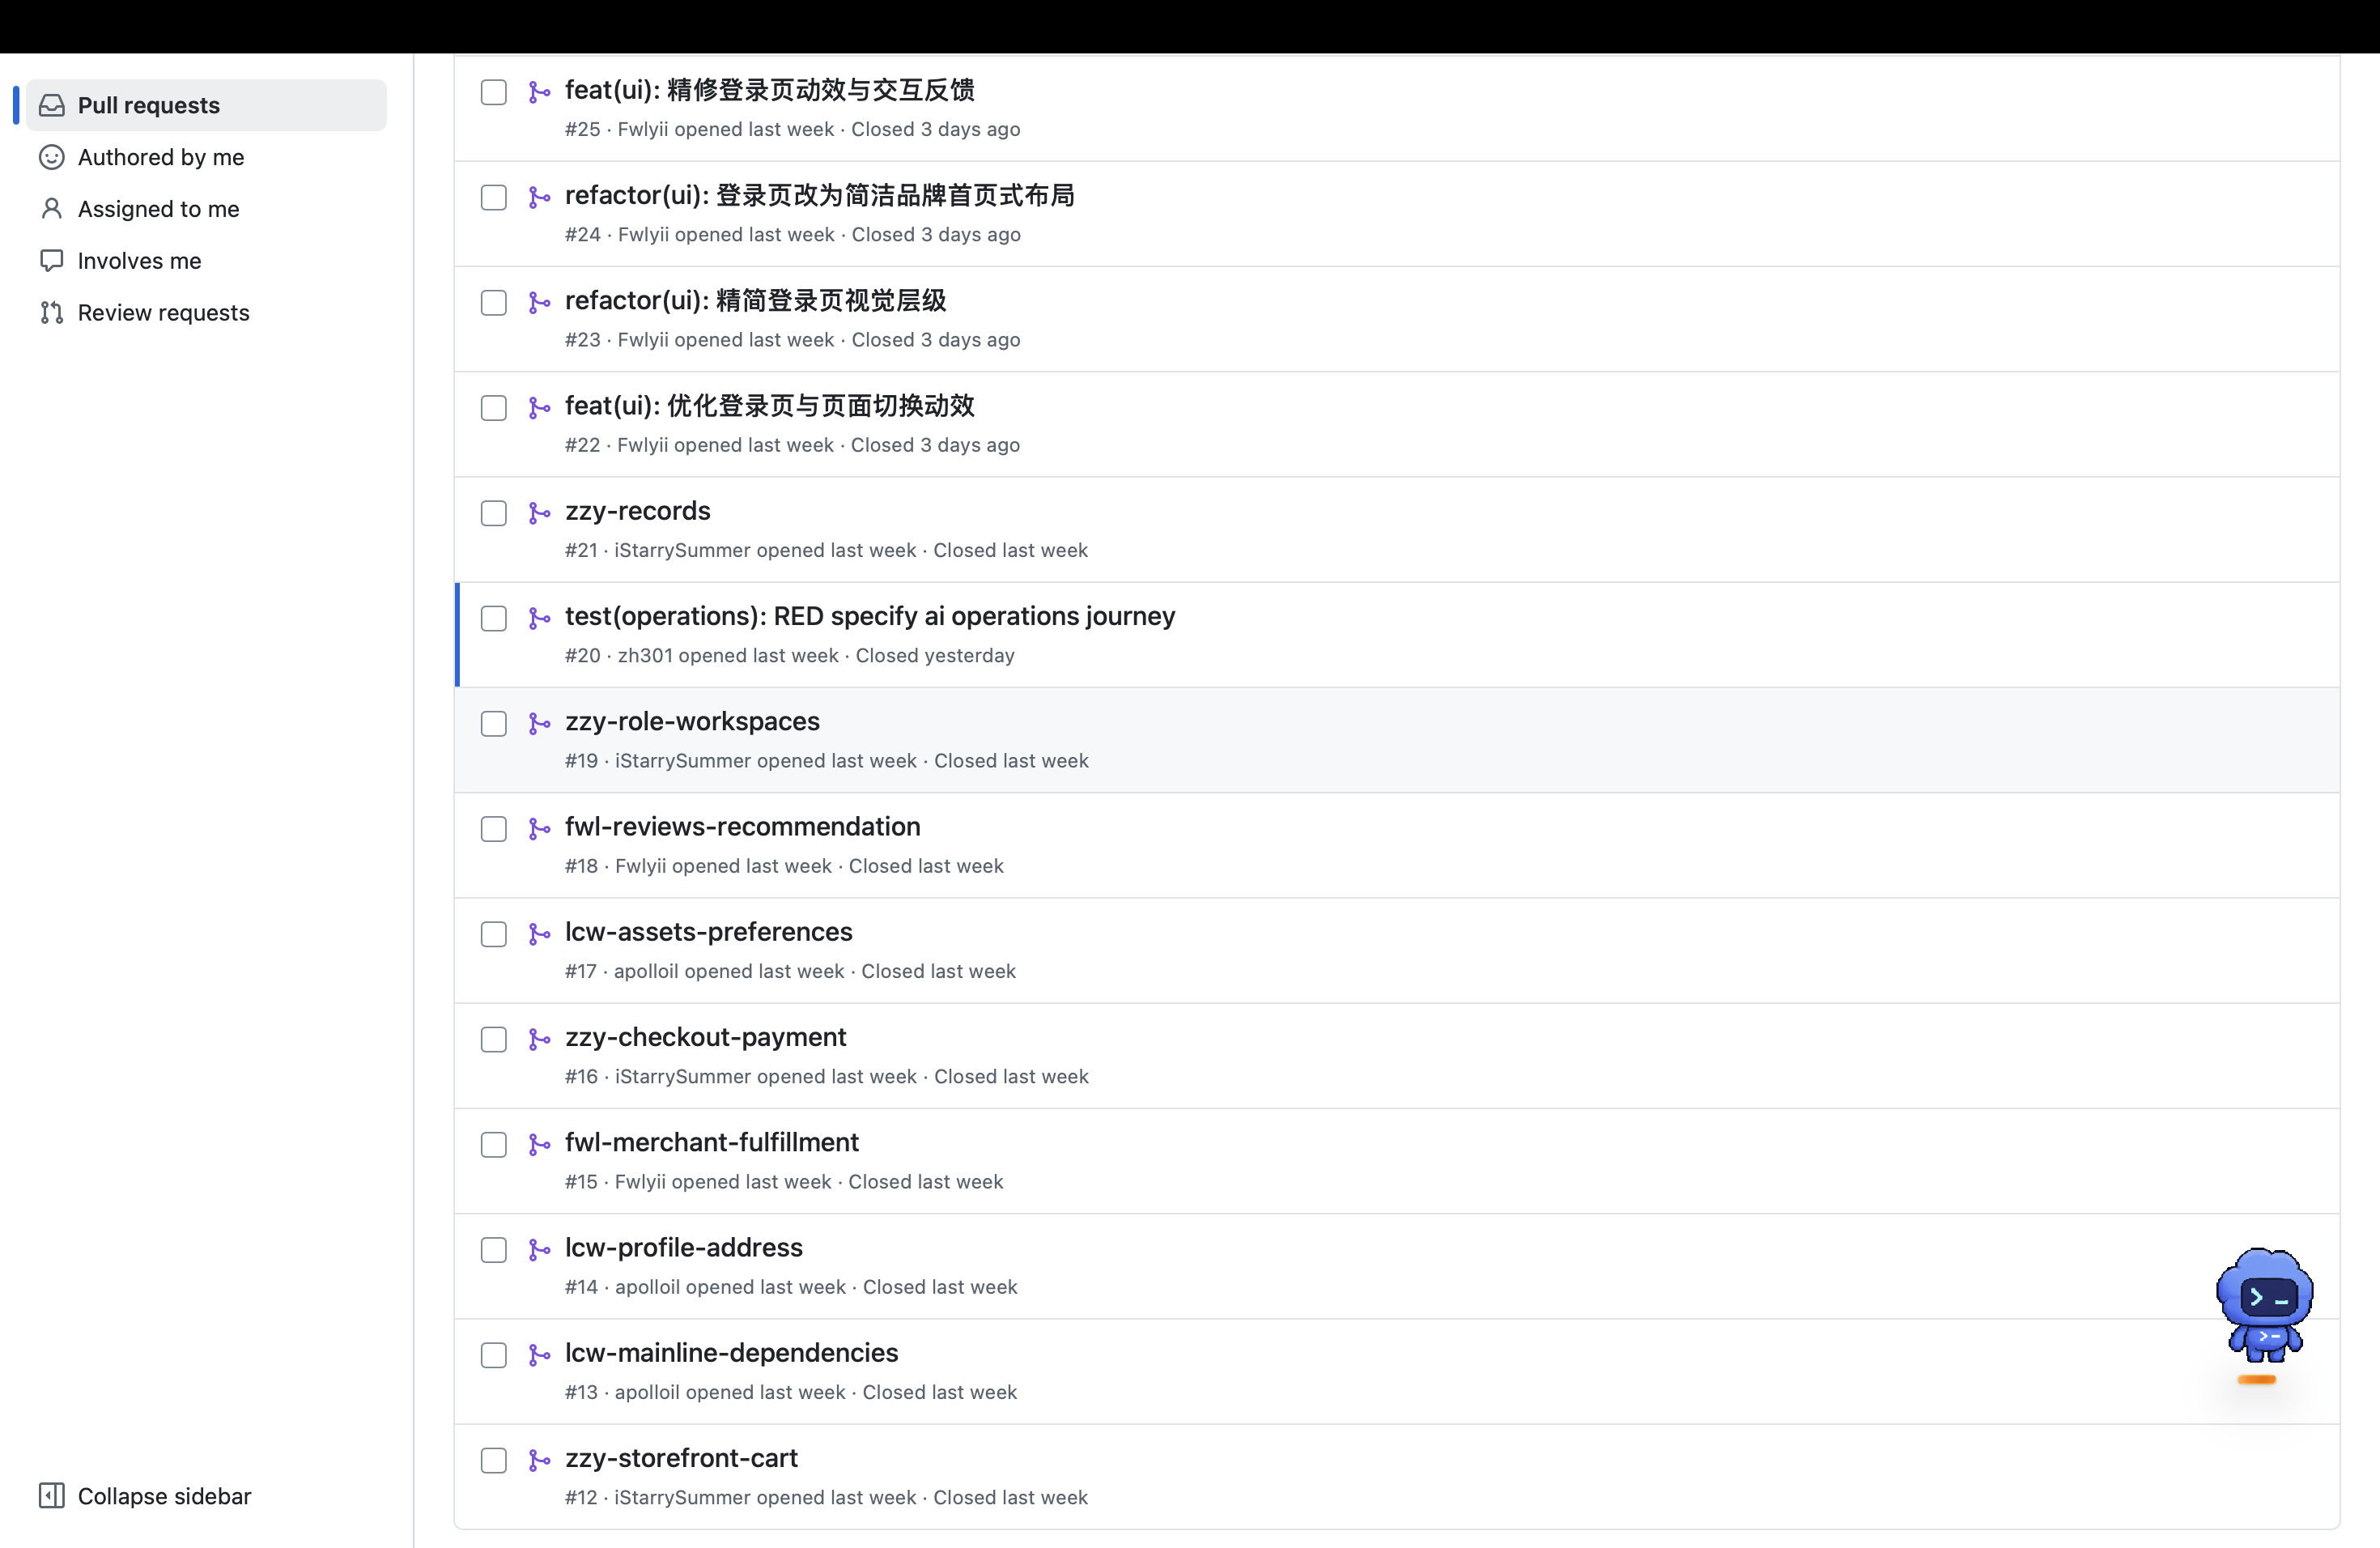
\includegraphics[width=\linewidth,height=.23\textheight,keepaspectratio]{figures/report/process/pull-requests.png}
    \captionof{figure}{团队累计 34 个 Pull Request 评审与合入记录截图}\label{fig:proc-prs}
  \end{minipage}
\end{figure}

GitHub 概览列出 227 条普通提交，其中 220 条进入主分支。全分支统计计入 38 条合并提交，共 265 条。PR 列表按合入请求记录结算支付、商家履约和登录动效等工作，可据此追查具体改动所属的版本。

图~\ref{fig:proc-git-daily} 按日期汇总全分支去重后的提交。9 月 3 日有 60 条，集中于 SRS 和建模。9 月 7 日有 35 条，集中于认证和环境编排。9 月 15 日有 28 条，对应封板整合。用图定位集中修改的日期，再通过 PR 查明改动内容，最后沿同一笔订单走查四端，\mbox{并核对回归结果}。

\begin{figure}[H]
  \centering
  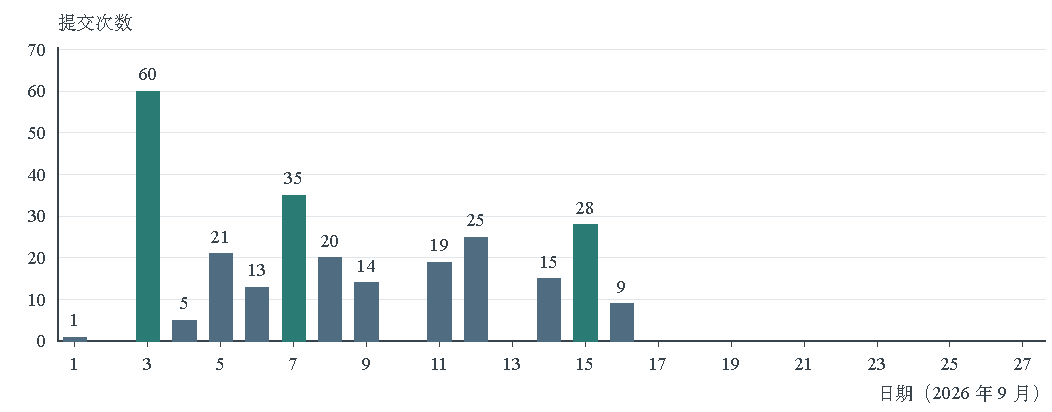
\includegraphics[width=.92\linewidth,height=.32\textheight,keepaspectratio]{figures/report/git-daily.pdf}
  \caption{项目周期每日 Git 提交频次分布统计图（9 月 1 日--9 月 27 日）}
  \label{fig:proc-git-daily}
\end{figure}
